\documentclass[12pt,a4]{report}
\usepackage{graphicx}

\begin{document}
	\title{%
		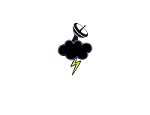
\includegraphics[scale=1.5]{mobicharged.png}~\\
		Project MobiCharged: Developement Process}
	\author{Team Super Charged (No.33)\\Nashit Mohammad - mohamn31\\Eric Nguyen - nguyee13\\Samuel De Haan - dehaas1\\Eamon Earl - earle2\\Mustafa Choueib - choueibm}
	\date{March 7th 2023 (R.1)}
	
\maketitle

\begin{document}
\newpage

\begin{center}
	\begin{table}
		\caption{\bf Revision History}
		\begin{tabular}{p{2cm}p{3cm}p{2cm}p{6cm}}
			\hline
			\bf Author & \bf Date & \bf Version & \bf Description\\
			\hline
			All & September 24, 2022 & Rev 0 & Created first draft of document\\
			\hline
			Nashit & March 7, 2023 & Rev 1 & Updated title, revision history and applied feedback from Rev 0\\
			\hline
		\end{tabular}
	\end{table}
\end{center}

\clearpage

\section*{Team Meeting Plan}
In order to produce a successful project, it is crucial that members of Team SuperCharged meet periodically at a timely manner to ensure the continuous production \& communication for Project MobiCharged. 

The team has concluded that a weekly meeting shall be sufficient. It is intended to be held every Monday at 7:30 PM virtually through the means of Discord and/or Microsoft Teams. The team has also finalized to hold a time slot to meet with the project supervisor. Based on the team’s availabilities as well as the supervisor’s, it had been concluded that meeting virtually on Sundays at 8:00 PM would suit all parties best. 

To make certain that meetings are indeed productive, it has been discussed that these meetings will follow a particular agenda. The first portion (roughly five – ten minutes) are reserved for off-topic discussions to build relations between project members. The second portion is to discuss upcoming deadlines. This way, all team members are up-to-speed regarding deliverables so they can begin generating ideas and/or discuss their preferred roles. The third portion of the meeting is for the team to communicate what has been completed so far, any challenges they are facing, any success-stories, etc. This will allow the team to get a better understanding of where we are in the project, which will significantly enhance the understanding of other members. This will also allow members who are struggling with any particular issues to be potentially assisted as other team members may be able to assist them whether it be through guidance or be able to completely join them in their tasks. It will also generate discussions between different team departments (for example: software and hardware) so they may be able to communicate when the integration occurs. In addition, the team will later discuss next steps as well as conclude the meeting. This agenda format can be summarized as shown:\\

\noindent Off-topic Discussions – Estimated 5-10 Minutes\\
Upcoming Deadlines – Estimated 5 Minutes\\
Current Statuses – Estimated 10-20 Minutes\\
Next Steps – Estimated 10-15 Minutes\\
Conclusion – Estimated 2-5 Minutes\\

In addition to the meeting agendas, a successful meeting will be held by assigning general roles to individuals during these meetings. These roles can be as shown below:\\

\noindent Meeting Conductor – Eamon\\
Meeting Concluder / Summarizer – Nashit\\
Meeting Note Taker – Eamon\\

It has been discussed that to limit the distractions going on during these meetings, only two individuals should be assigned roles during these meetings so that the group may focus during these discussions. The conductor will primarily ensure the meeting follows the agenda and limits distractions that exceed an acceptable amount. The concluder will be assigned the role of concluding the meeting by summarizing what has been discussed, as well as discuss “homework”. Finally, the note taker will simply note the conclusions made by the concluder and post them in the general chat of the party so that every member is clearly aware of their responsibilities. 

\section*{Team Communication Plan}
It has been finalized that the main course of communication will be through Discord. Developers are expected to reach out to the group on Discord should they need help with their ticket, or simply to discuss logistics. They should be accessible on Discord during work hours. Moreover, the phone numbers of all parties have been pinned for future reference in the scenario that last resort time-sensitive communication needs to be conducted. Discord allows the ability of assigned custom roles, schedule meetings, create separate channels for separate tasks and much more, which the team found extremely viable for our project. 

\section*{Team Member Roles}
As with any successful group, there are assigned member roles to indicate which tasks get assigned to which members. Below is the general member roles along with who it is assigned to: \emph{*note that roles are flexible and are not concrete. Roles are adaptable as some may be added and/or removed.}\\

\noindent \textbf{Supervisor Liaison:} Eamon\\
This role is designed to be the main point of contact between the supervisor and remaining members.\\

\noindent \textbf{General Project Manager:} Nashit\\
The general project manager is to overview the project, ensure effective communication between teams, revise steps if necessary and assist teams when possible.\\

\noindent \textbf{Software Architectural Design:} Mustafa (Primary) \& Eamon (Secondary)\\
The goal of the software architect designers is to create the design of the programs on a surface level as well as be responsible for the process of integration between software programs / codes.\\

\noindent \textbf{Machine Learning Developer:} Eric\\
The primary task at hand for the machine learning developer is to apply the skills of machine learning in order to produce the code necessary for successful software. The machine learning developer will work closely with the software architectural design team as well as the developers.\\

\noindent \textbf{Software Developers:} Mustafa (Primary), Eric \& Eamon (Secondary)\\
The role of the software developers is to produce generic code (that does not constitute as machine learning) for the purpose of front-end \& back-end development.\\

\noindent \textbf{Researcher:} Nashit (Primary) \& Sam (Secondary)\\
This role is for the purpose of generating key notes and building an understanding of the technologies involved as well as the physics behind the creation of this project.\\

\noindent \textbf{Documentation / Reporting:} Nashit\\
In order to hand in deliverables as well as produce notes for the team, this role is the team-lead when producing the necessary reports on a timely manner.\\

\noindent \textbf{Prototype Engineer:} Sam\\
The prototype engineer will be the main individual to generate the prototype as well as assign tasks to assisting members in order for production. This individual will work closely with the software architectural design team as well as the research team.

\section*{Workflow}
The process workflow that will be implemented will prioritize the feature branch workflow. This allows for multiple developers to work on specific aspects of the project with ease. This workflow provides an advantageous element for continuous integration and allows for thorough review from other developers prior to changes/additions being integrated into the main project. In combination with issues \& labels, isolation of bugs, necessary changes/fixes, and unfinished tasks, become very simple. 

This workflow will consist of a main branch (only fully functioning, tested / reviewed, and complete code will exist in this branch) in which developers will start by pulling all changes. This will provide a local copy of the current state of the remote repository. The team will then convene on a weekly basis to generate issues/tickets that will consist of a detailed description identifying what is required from the issue and all the information necessary for other developers to understand the objective of the issue. Each issue will also have associated labels that will indicate the nature of the issue (bug fixes, new feature, modifications, etc.,), as well as their respective priorities (high or low priority). Any additional issues or labels discovered will be created during this weekly cycle. The issues will be assigned to a developer that is best fit to complete them. 

From this point, features or bug fixes will require a new branch to be created and developers will complete the task necessary in that branch. This entails committing code to the new branch with descriptive, yet concise, commit messages that effectively detail the nature of the commit. Commit messages should also include any issue numbers that are relevant to the changes made at the end of the message. Once the code is complete and has been committed/pushed to the branch, the developer will conduct a pull request that denotes the commit is ready to be reviewed. After the pull request is opened, a developer independent of the author of the pull request will manually review that code to ensure the requirements detailed in the created issue have been met. 

Alongside this, the developer is required to create test cases (during development) that will be used by the reviewer to determine whether the code meets the intended requirements. It is up to the discretion of the reviewer to decide whether the number of test cases created by the developer is satisfactory relative to the behavioral changes of the pull request (edge-covering). Tests will be run automatically using GitHub Actions, which will prevent any pull requests from being merged into the main branch without passing every test case provided. 

Once the reviewer approves of the changes, ensures the requirements have been fully met for the respective issue and ensures the code is linted and up to the formatting standard required, the branch will be merged into the main branch by the developer. Proceeding the merge to the main branch, the developer will then close the respective issue.\\

\noindent A quick summary of the workflow described above:\\

\noindent 1.	Pull all changes from the main branch.\\
\noindent 2.	Create any necessary branches for features or bug fixes.\\
\noindent 3.	Continuously commit code and the necessary test suite\\
\noindent 4.	Create a pull request once code is complete\\
\indent a.	GitHub actions will run the automated tests\\
\indent \indent  i.	Must pass all tests, otherwise will not be merged.\\
\indent b.	Independent review of the code to ensure the requirements have been met.\\
\noindent 5.	Developer will merge into the main branch and close the respective issue.\\


\section*{Proof of Concept Demonstration Plan}
Proof of concept will be demonstrated through the improvement generated by the developed algorithm (as compared to the current method of manually conducting simulations). The machine learning algorithm’s output will be compared to that of a pre-existing configuration to determine the degree of effective performance increase. 

While physical implementation may pose a significant risk for a real-time demonstration, the proof of concept can be demonstrated via simulation results. Comparison between simulation results and post optimization through the developed algorithm will work as means to show improved and desired results during demonstration.

Another risk lies in procurement of all the variations of hardware components. Various, more sophisticated, hardware components may not be available to test and validate in a real-world practical means due to limited supply. This again will be overcome through simulation validation. 

The hardware portion of the prototype created holds the largest risk when meeting the deadline of the Proof of Concept Demonstration as the procurement of parts and creation of design will be difficult to meet based on the deadline. As a result, the team at the very least will create a chart displaying the parts required (verifying the effort in planning) and discuss the idea of the prototype. This prototype will be used to either gather real life data that can be sent to the machine learning algorithm for verification purposes or be simply used as a demonstration tool that may also be implemented in classes for the purposes of teaching.

Ultimately, a working and physical prototype along with simulation results will be available for proof of concept during demonstration. The extent of the prototype sophistication will be determined as the project progresses.

\section*{Technology}
The current plan for which technologies are to be implemented are as follows:\\

\noindent \textbf{Matlab:}\\
\noindent Matlab will be implemented for the process of generating simulations and collecting data.\\

\noindent \textbf{Python:} TensorFlow and/or PyTorch, Matplotlib\\
\noindent These libraries will be used to build, train, and evaluate the machine learning models that will be used in this project. Matplotlib will be used to display the performance of the trained models.\\

\noindent \textbf{Pylint:}\\
\noindent Pylint will be the intended linter for usage which aligns with the PEP8 style coding guide intended for use.\\

\noindent \textbf{Golang:}\\
\noindent Golang is in plan of being implemented for the usage of concurrency control due to the current generic model of the system. 

\section*{Coding Styles / Standards}
The intended coding style that will be applied for this project is PEP8. This will also align with the Pylint linter for the linting of our code. 

After discussion amongst the team, it was deemed that a few standards were important for the success of the project. One priority is to make the methods self-descriptive, in which it is easily understood by descriptive variable names and easy-to-read coding structures (which of course stands with some exceptions). The key idea is to include comments when necessary, but to limit them in the sense that they are redundant if the code is already self-descriptive. Another priority was any method should only do one task. In terms of abstracted coding styles the goal is to prioritize designing for change in the expectation that the pieces we integrate with (like the simulation) will increase in efficiency and I/O speed in the future. As such we also want to prioritize modularity, so that pieces can be swapped and upgraded with relative ease and of course prioritizing the efficiency of our own main algorithms as well. There will be a good balance between the drive for efficiency with the current speed restrictions that pre-exist, and our budget / hardware restrictions. This implies flexible code that can scale up in its throughput, implying that we should focus on concurrency and our program making full use of its downtime.

\section*{Project Scheduling}
The project will be scheduled with major milestones as follows:\\

\noindent 1.	Reading up on the technology and the physics involved in a phase array.\\
\noindent 2.	(In parallel with 1) Do investigation on the client's current optimization system, and how we can get more data out of it. Also, to learn about their current server system to perfect and specify abstract design mock-ups.\\
\noindent 3.	Build an end-to-end data processing pipeline (bare bones), and the associated databases.\\
\noindent 4.	Build the antennae array.\\
\noindent 5.	Assess error of their current simulation using the physical model and scientific computing principles.\\
\noindent 6.	Build deep learning program (the first half – in taking and learning from the simulation data).\\
\noindent 7.	Build the ‘initiative element’. The second half of the deep learner that will drive ‘explorative simulation’. \\
\noindent 8.	Develop concurrency and priority monitor for these two separate functionalities.\\
\noindent 9.	Let it learn (procure an environment for it the program to take in the data and run in the background, while we work to improve it). This step may require a reconsideration of our database size.\\
\noindent 10.	Work on multi-threading or running the simulation on multiple machines.\\
\noindent 11.	(Stretch goal) Improve the speed of their current simulation.\\

To make the resources of the team as most efficient as possible, the weekly meetings will be advantageous as members will be able to discuss the tasks at hand as well as assign tasks to the best suitable individuals. 

\end{document}


	
	